\section{Auswertung}
\label{sec:Auswertung}

\subsection{Bestimmung der Winkelrichtgröße}

Die aufgenommen Messdaten zur Bestimmung der Winkelrichtgröße sind in Tabelle \ref{tab:Messdaten1}
zu finden. Dabei wurde die Kraft bei verschiedenen Auslenkwinkeln $\varphi$ gemessen. Der Hebelarm
hat die konstante Länge \SI{0.3}{\meter}.

\begin{table}
\centering
\caption{Ausgelenkter Winkel mit dazugehöriger Kraft}
\label{tab:Messdaten1}
\sisetup{table-format=2.1}
\begin{tabular}{c c c c}
\toprule
$Winkel \,/\, °$ & $Winkel \,/\, rad$ & $F \,/\, \si{\milli\newton}$ & $M \,/\, \si{\milli\newton\meter}$\\
\midrule
 35 & 0.61 &  30 &  9.00\\
 45 & 0.79 &  35 & 10.05\\
 50 & 0.87 &  40 & 12.00\\
 55 & 0.96 &  50 & 15.00\\
 60 & 1.05 &  55 & 16.50\\
 70 & 1.22 &  61 & 18.30\\
 80 & 1.40 &  83 & 24.90\\
 90 & 1.57 & 102 & 30.60\\
100 & 1.66 & 110 & 32.40\\
 95 & 1.74 & 108 & 33.00\\
\bottomrule
\end{tabular}
\end{table}

Anhand von Formel \eqref{eqn:Winkelrichtgröße} ist zu erkennen, dass die Winkelrichtgröße $D$ 
lediglich ein Proportionalitätsfaktor zwischen Drehmoment $M$ und Winkel $\varphi$ ist. Zur Ermittlung 
dieser Größe wird eine lineare Regressions mittels python und matplotlib durchgeführt. 
Das Ergebnis ist in Abbildung \ref{fig:plot1} zu sehen. 


\begin{figure}
  \centering
  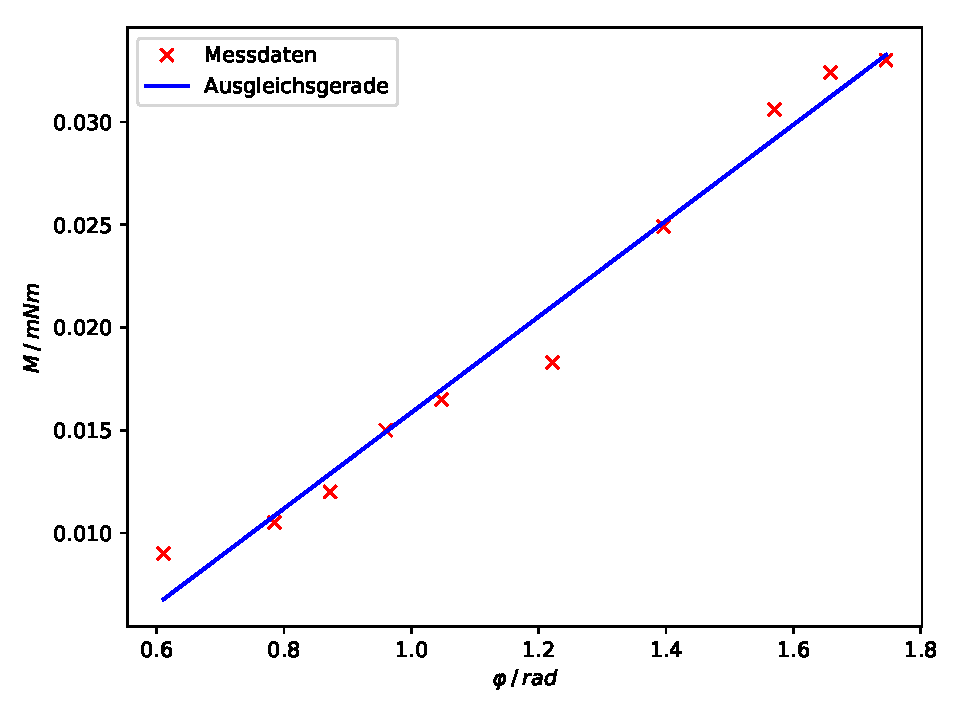
\includegraphics[scale=0.8]{content/plot1.pdf}
  \caption{Darstellung des Zusammenhanges zwischen M und $\varphi$}
  \label{fig:plot1}
\end{figure}

Die Ausgleichsgerade ist gegeben mit $M(\varphi) = a\cdot \varphi + b$. Für die Regressionsparameter
ergibt sich: 

\begin{align*}
a &= \SI{23.34+-1.43}{\milli\newton\meter} \\
b &= \SI{-7.5+-1.78}{\milli\newton\meter}
\end{align*}

Der Steigungsfaktor $b$ entspricht dabei der Winkelrichtgröße $D$. Somit ergibt sich: 

\begin{equation*}
D = \SI{23.34+-1.43}{\milli\newton\meter}
\end{equation*}

\subsection{Bestimmung des Trägheitsmoments der Drillachse}

Zur Bestimmung des Eigenträgheitsmoments der Drillachse wird die Periodendauer $T$ in Abhängigkeit 
des Abstands $a$ der Gewichte zur Drillachse gemessen. Die erhaltenen Daten sind in Tabelle 
\ref{tab:Messdaten2} aufgeführt. Dabei ist $T_7$ die gemessene Dauer für 7 Perioden.

\begin{table}
\centering
\caption{Messwerte zum Trägheitsmoment der Drehachse}
\label{tab:Messdaten2}
\sisetup{table-format=2.1}
\begin{tabular}{c c c c c}
\toprule
$a \,/\, \si{\meter}$ & $a² \,/\, m²$ & $T_7\,/\, \si{\second}$ & $T \,/\, \si{\second}$ & $T² \,/\, s²$\\
\midrule
 0.2700 & 0.0729 & 57.93\,\pm 0.5 & 8.28\,\pm 0.071 & 68.49\,\pm 1.18\\
 0.2300 & 0.0529 & 50.30\,\pm 0.5 & 7.19\,\pm 0.071 & 51.63\,\pm 1.03\\
 0.2090 & 0.0437 & 46.89\,\pm 0.5 & 6.70\,\pm 0.071 & 44.87\,\pm 0.96\\
 0.1885 & 0.0355 & 43.00\,\pm 0.5 & 6.14\,\pm 0.071 & 37.73\,\pm 0.88\\
 0.1695 & 0.0287 & 40.10\,\pm 0.5 & 5.73\,\pm 0.071 & 32.82\,\pm 0.82\\
 0.1490 & 0.0222 & 35.72\,\pm 0.5 & 5.10\,\pm 0.071 & 26.04\,\pm 0.73\\
 0.1295 & 0.1677 & 32.58\,\pm 0.5 & 4.65\,\pm 0.071 & 21.66\,\pm 0.66\\
 0.1090 & 0.0119 & 28.85\,\pm 0.5 & 4.12\,\pm 0.071 & 16.99\,\pm 0.59\\
 0.0890 & 0.0079 & 25.49\,\pm 0.5 & 3.64\,\pm 0.071 & 13.26\,\pm 0.52\\
 0.0690 & 0.0048 & 22.36\,\pm 0.5 & 1.19\,\pm 0.071 & 10.20\,\pm 0.46\\
\bottomrule
\end{tabular}
\end{table}

Aus \eqref{eqn:Steiner} und \eqref{eqn:Periode} folgt der Zusammenhang: 

\begin{equation*}
T² = \underbrace{\frac{4\pi²m}{D}}_{\hat = s}\cdot a² + \underbrace{\frac{4\pi²}{D} I_D}_{\hat = b}
\label{eqn:Regression}
\end{equation*}

Mittels linearer Regression wird nun der als $b$ bezeichnete Parameter 
ermittelt und daraus das gesuchte Trägheitsmoment $I_D$ berechnet. Das 
Ergebnis ist in Abbildung \ref{fig:plot2} dargestellt. 

\begin{figure}
  \centering
  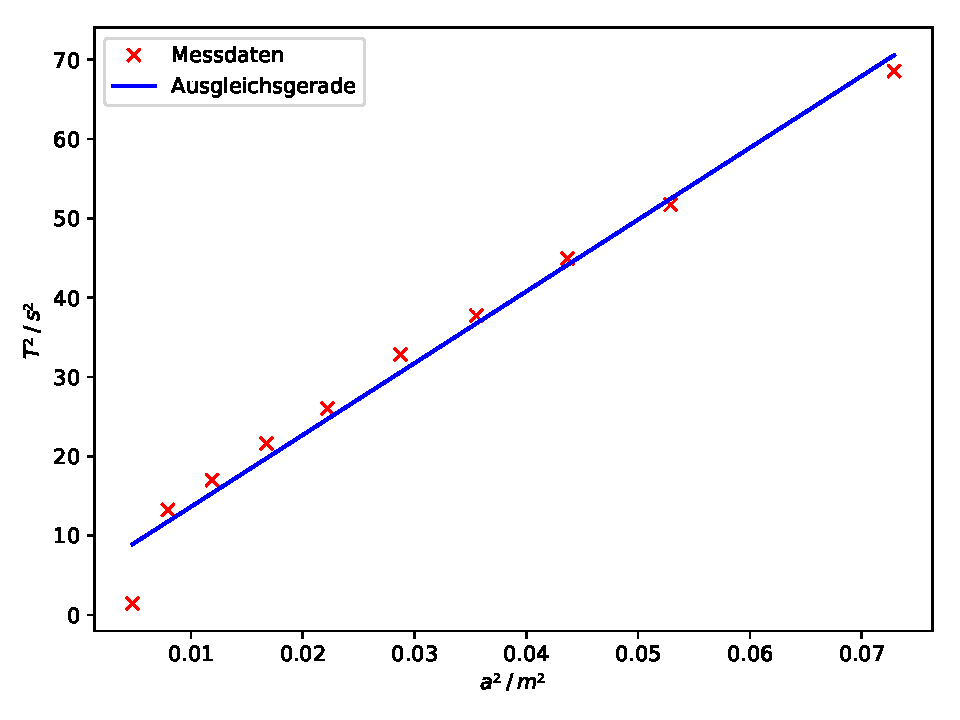
\includegraphics[scale=0.8]{content/plot2.pdf}
  \caption{$T²$ gegen $a²$ aufgetragen mit eingezeichnetere Regression}
  \label{fig:plot2}
\end{figure}

Die Parameter der Ausgleichsgerade ergeben sich zu: 

\begin{align*}
s &= \SI{905.17+-54.89}{\second²\per\meter²}\\
b &= \SI{4.59+-1.99}{\second²}
\end{align*}

Damit berechnet sich $I_D$ zu: 

\begin{equation*}
I_D = \frac{b\cdot D}{4\pi²} = \SI{2.7+-1.2e-3}{\kilo\gram\meter²}
\end{equation*}

Der statistische Fehler berechnet sich dabei mit der Gaußschenfehlerfortpflanzung 
zu: 

\begin{equation*}
\Delta I_D = \sqrt{\left(\frac{\partial I_D}{\partial b}\cdot \Delta b\right)²+\left(\frac{\partial I_D}{\partial D}\cdot \Delta D\right)²}
= \sqrt{\left(\frac{D}{4\pi²}\cdot \Delta b\right)²+\left(\frac{b}{4\pi²}\cdot \Delta D\right)²}
\end{equation*}

\subsubsection{Verifikation des Satzes von Steiner}

Anhand der Daten, die zur Ermittelung des Eigenträgheitsmoments $I_D$ berechnet wurden, lässt sich der
Satz von Steiner verifizieren. Die verwendete Regressionsformel \eqref{eqn:Regression} folgt unter der
Annahme, das der Steiner'sche Satz gilt. Diese Formel fordert einen linearen Zusammenhang zwischen 
$T²$ und $a²$. Wie in Abbildung \ref{fig:plot2} zu erkennen ist, lässt sich dieser Zusammenhang 
bestätigen. Die Geradensteigung

\begin{equation*}
s = \SI{905.17+-54.89}{\second²\per\meter²}
\end{equation*}

passt ebenfalls zu dem theoretischen Wert, der sich mit der Gesamtmasse der Gewichte  $m = 2\cdot 
\SI{0.2218}{\kilo\gram}$ eingesetzt in die Definition von $s$ in Formel \eqref{eqn:Regression} zu 
dem Wert:

\begin{equation*}
s_{theo} = \SI{750+-50}{\second²\per\meter²}
\end{equation*}

ergibt.
Dabei ist der Fehler des theoretischen Wertes gegeben durch:

\begin{equation*}
\Delta s = \frac{-4\pi²m}{D²} 
\end{equation*}

\subsection{Trägheitsmomente zweier einfacher Körper}

Die zu untersuchenden Körper werden oben auf der Drillachse befestigt, zum Schwingen gebracht 
und die Periodendauer $T$ gemessen. Es werden zwei Körper untersucht: Ein Zylinder und eine Kugel.
Diese Körper besitzen folgende Maße: 

\begin{align*}
m_Z &= \SI{1005.9}{\gram}\\
d_Z &= \SI{7.95+-0.05}{\centi\meter}\\
m_K &= \SI{812.4}{\gram}\\
r_K &= \SI{7.5+-0.05}{\centi\meter} 
\end{align*}

Die ermittelten Periodendauer und Trägheitsmomente finden sich in Tabelle \ref{tab:Messdaten3}.

\begin{table}
\centering
\caption{Messwerte Kugel und Zylinder}
\label{tab:Messdaten3}
\sisetup{table-format=2.1}
\begin{tabular}{c c c c}
\toprule
\multicolumn{2}{c}{Zylinder} &  \multicolumn{2}{c}{Kugel} \\
\midrule
$T_Z \,/\, \si{\second}$ & $I_Z \,/\, \SI{1e-3}{\kilo\gram\meter²}$ & $T_K\,/\, \si{\second}$ & $I_K \,/\, \SI{1e-3}{\kilo\gram\meter²}$\\
\midrule
 1.21\,\pm 0.07 & 0.862\,\pm 0.115 & 1.73\,\pm 0.71 & 1.769\,\pm 0.182\\
 1.14\,\pm 0.07 & 0.770\,\pm 0.107 & 1.69\,\pm 0.71 & 1.691\,\pm 0.176\\
 1.15\,\pm 0.07 & 0.782\,\pm 0.108 & 1.73\,\pm 0.71 & 1.767\,\pm 0.182\\
 1.15\,\pm 0.07 & 0.782\,\pm 0.108 & 1.66\,\pm 0.71 & 1.629\,\pm 0.172\\
 1.16\,\pm 0.07 & 0.196\,\pm 0.109 & 1.69\,\pm 0.71 & 1.686\,\pm 0.176\\
\midrule
\multicolumn{2}{c}{$\bar{I_Z}= \SI{0.80+-0.07}{\kilo\gram\meter²}$} & \multicolumn{2}{c}{$\bar{I_K} = \SI{1.71+-0.12}{\kilo\gram\meter²}$} \\
\bottomrule
\end{tabular}
\end{table}

Dabei ergeben sich die Fehler der Trägheitsmomente zu: 

\begin{equation*}
\Delta I = \sqrt{\left(\frac{\partial I}{\partial T}\cdot \Delta T\right)²+\left(\frac{\partial I}{\partial D}\cdot \Delta D\right)²}
= \sqrt{\left(\frac{T D}{2\pi²}\cdot \Delta T\right)²+\left(\frac{T²}{4\pi²}\cdot \Delta D\right)²}
\end{equation*}

Nun werden die theoretischen Trägheitsmomente der beiden Körper berechnet, um die 
experimentell ermittelten Daten mit diesen zu vergleichen. Die Trägheitsmomente 
der Kugel, bzw. des Zylinders werden hierbei mit den bekannten Formeln berechnet:

\begin{align*}
I_{K, theo} &= \frac{2}{5} mR²\\
I_{Z, theo} &= \frac{1}{2} mR²
\end{align*}

Mit den Maßen der verwendeten Körper ergeben sich somit: 

\begin{align*}
I_{K, theo} &= \SI{1.828+-0.024}{\kilo\gram\meter²}\\
I_{Z, theo} &= \SI{0.795+-0.010}{\kilo\gram\meter²}
\end{align*}

Die experimentell bestimmten Trägheitsmomente weichen von den theoretischen
Werten um $\SI{6.9}{\percent}$ bei der Kugel und um $\SI{0.625}{\percent}$ bei dem Zylinder ab.

\subsection{Trägheitsmoment einer Puppe in zwei Stellungen}